\chapter{Results}
\label{chapter:results}
\gls{NCLT} dataset was used for the comparison of different filters. Functionality of each component has been tested with \gls{KITTI}, \gls{KAIST} and \gls{NCLT} datasets.



%%%%%%%%% ch start %%%%%%%

\section{Comparison of Bayesian filters}
\label{sec:BayesianFilterComparison}
Data from the \gls{NCLT} dataset has been used for this comparison and the results shown in the discussion have been obtained using sequence 2013.01.10.
\subsection{Performance of translation estimation}
Overall performances (\gls{RMS} error) of all the filters are better than the raw \gls{GNSS} measurements. \gls{UKF} has given the worst estimation while \gls{PF} and \gls{ESKF} have given better results. Table \ref{table:ch:RMSErrorPosition} shows a summary of the results.
\begin{table}[h]
    \centering
    \begin{tabular}{|p{2.5cm}|p{2.5cm}|p{2.5cm}|p{2.5cm}|p{2.5cm}|} 
        \hline
        \textbf{Method} & \textbf{x} & \textbf{y} & \textbf{z}& \textbf{Overall} \\
        \textbf{} & \textbf{direction(m)} & \textbf{direction(m)} & \textbf{direction(m)}& \textbf{position(m)} \\
        \hline
        GPS&6.3278 &9.8746 &5.6387& 13.0133\\
        \hline
        ESKF &4.6824& 2.8655 &7.0109 &8.9044\\
        \hline
        UKF &4.7371& 2.7663 &11.2554 &12.5211
        \\
        \hline
        PF& 4.4488& 2.8587& 6.8126& 8.6242
        \\
        \hline
    \end{tabular}
\caption{Translational \gls{RMS} errors for different Bayesian filters}
\label{table:ch:RMSErrorPosition}
\end{table}

Even though \gls{PF} has given the most accurate results, as shown in figures \ref{fig:ch:errorX} to \ref{fig:ch:errorPositionOverall}, output of the filter is not smooth. Furthermore, the estimate rapidly diverges upon receiving erroneous \gls{GNSS} measurements (see figure \ref{fig:ch:errorPositionOverall}). Adding random samples or increasing the size of the particle set are alternatives for this problem. However, both of these solutions will increase the computational complexity. If both \gls{RMS} error and smoothness are considered, \gls{ESKF} gives the best solution. Z-direction has shown the worst error in all the three filters resulting a large overall positional error. This behaviour is a result of the large error in the altitude measurement, obtained by the \gls{GNSS} receiver. It can be mitigated by using an Altimeter (which is only present in the \gls{KAIST} dataset, out of the three datasets being used).

\begin{figure}[h]
    \centering
    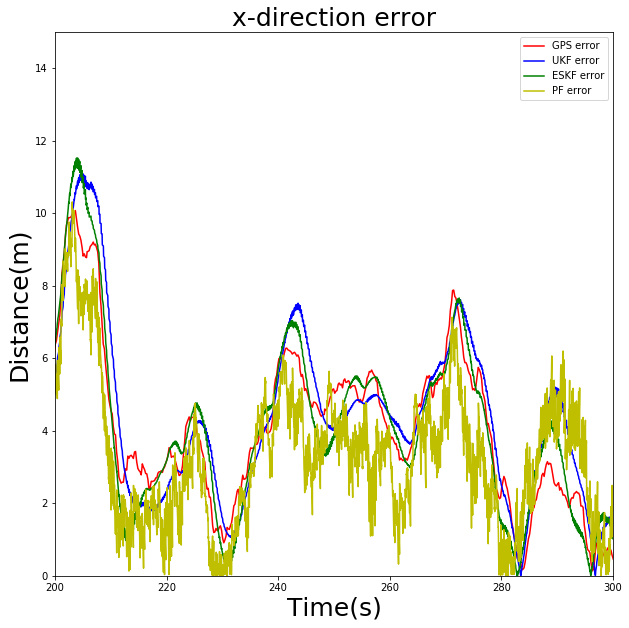
\includegraphics[width=0.7\textwidth]{figs/x_direction.png}
    \caption{Filter comparison - error in x direction}
    \label{fig:ch:errorX}
\end{figure}
\begin{figure}[h]
    \centering
    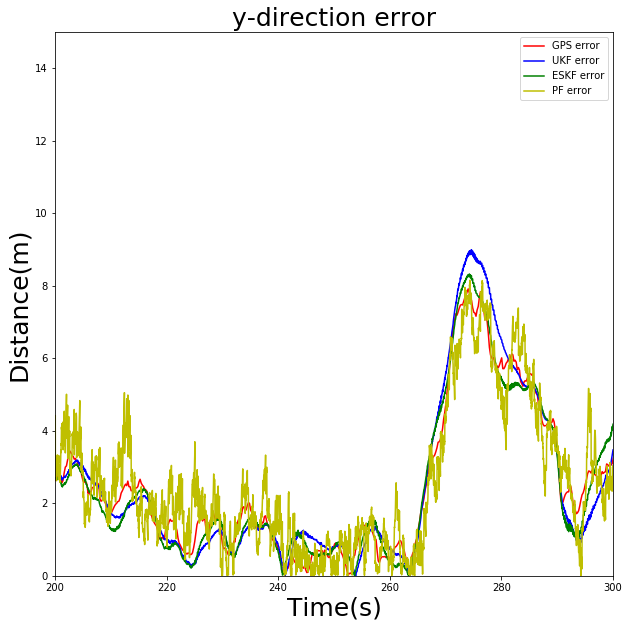
\includegraphics[width=0.7\textwidth]{figs/y_direction.png}
    \caption{Filter comparison - error in y direction}
    \label{fig:ch:errorY}
\end{figure}
\begin{figure}[h]
    \centering
    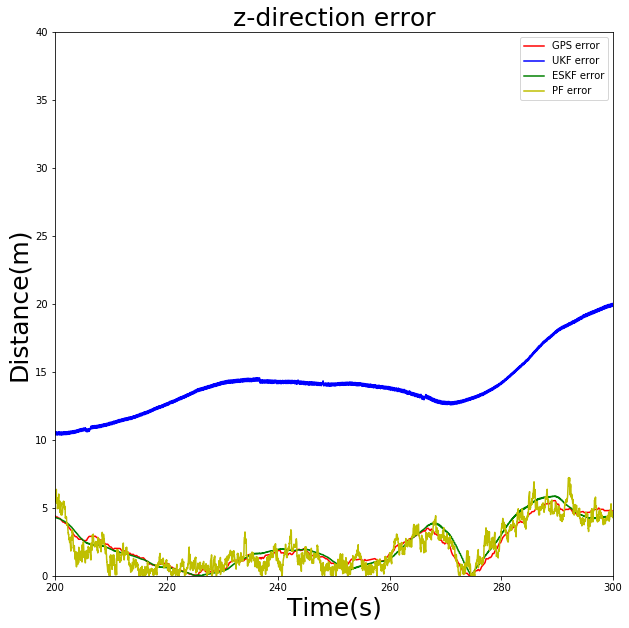
\includegraphics[width=0.7\textwidth]{figs/z_direction.png}
    \caption{Filter comparison - error in z direction}
    \label{fig:ch:errorZ}
\end{figure}
\begin{figure}[h]
    \begin{subfigure}{0.5\textwidth}
        \centering
        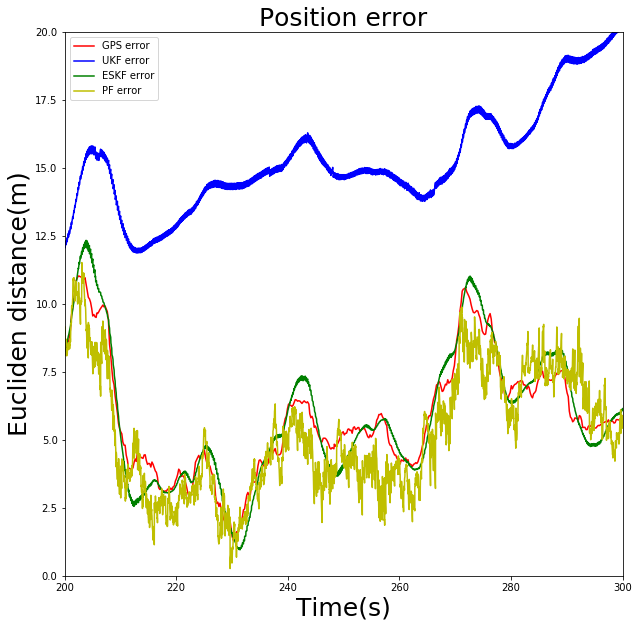
\includegraphics[width=1\textwidth]{figs/overall.png}
        \caption{Excluding the diverged \gls{PF} result}
    \end{subfigure}%
    \begin{subfigure}{0.5\textwidth}
        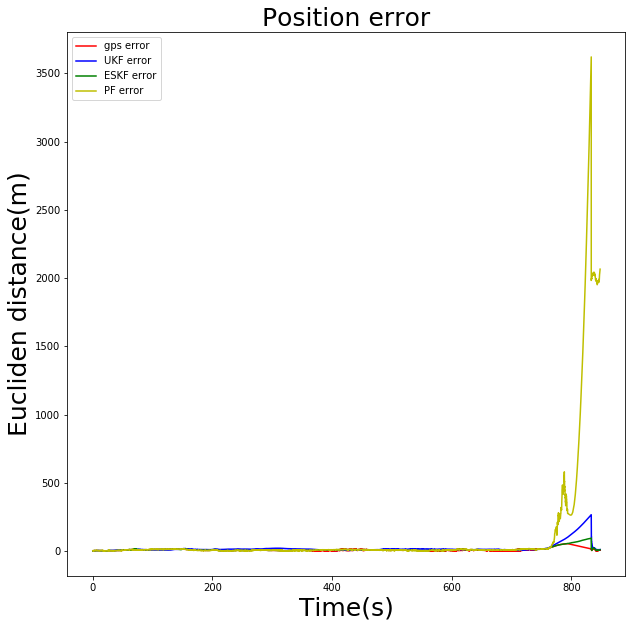
\includegraphics[width=1\textwidth]{figs/overall_diverge.png}
        \caption{Including the diverged \gls{PF} result}
    \end{subfigure}
    \caption{Filter comparison - overall translational error}
    \label{fig:ch:errorPositionOverall}
\end{figure}


\subsection{Performance of orientation estimation}
Raw orientation measurement obtained using the \gls{IMU} + Magnetometer is better than the estimates of all the three filters (see table \ref{table:ch:RMSErrorRotation}). This is due to the noise in the angular velocity measurement, which is confirmed from the reduction of the error when the angular measurement noise variance parameter is increased. \gls{PF} has given the worst estimation. Results of the other two filters are somewhat similar. However, \gls{UKF} has given the best
estimation. Error plots are shown in figures \ref{fig:ch:errorRoll}, \ref{fig:ch:errorPitch} and \ref{fig:ch:errorYaw}.
\begin{table}[h]
    \centering
    \begin{tabular}{|p{4cm}|p{3cm}|p{3cm}|p{3cm}|} 
        \hline
        \textbf{Method} & \textbf{Roll (deg)} & \textbf{Pitch (deg)} & \textbf{Yaw (deg)} \\
        \hline
        \gls{IMU}+Magnetometer & 1.1555 &1.7171 &7.7622\\
        \hline
        ESKF& 2.8258& 3.3362& 8.8584\\
        \hline
        UKF &1.7216& 1.8304& 8.6043
        \\
        \hline
        PF &14.76759& 12.32548 &37.5694
        \\
        \hline
    \end{tabular}
    \caption{Rotational \gls{RMS} errors of different Bayesian filters}
    \label{table:ch:RMSErrorRotation}
\end{table}

\begin{figure}[h]
\centering
	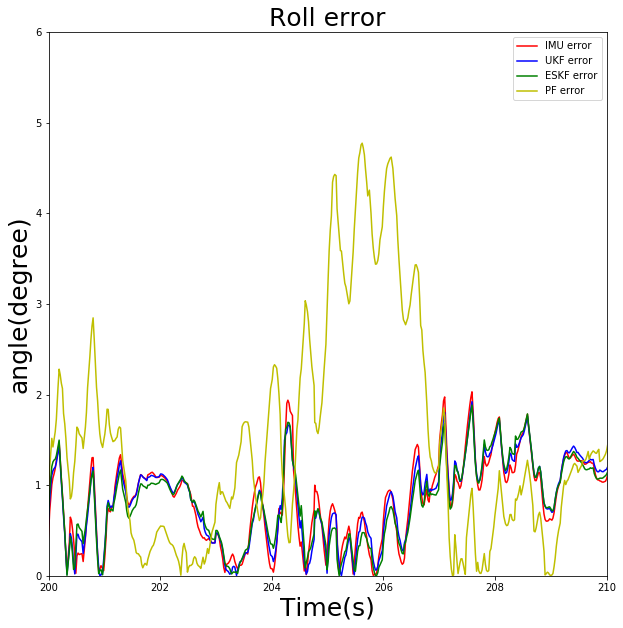
\includegraphics[width=0.7\textwidth]{figs/roll.png}
	\caption{Filter comparison - error in roll}
	\label{fig:ch:errorRoll}
\end{figure}

\begin{figure}[h]
\centering
	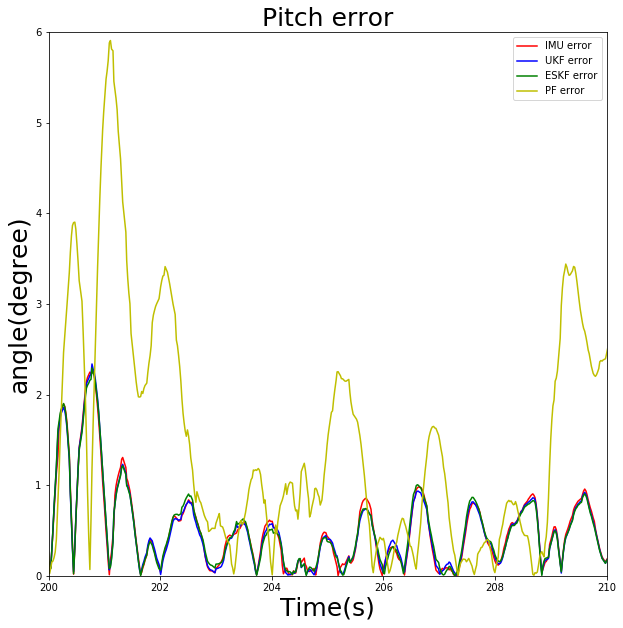
\includegraphics[width=0.7\textwidth]{figs/pitch.png}
	\caption{Filter comparison - error in pitch}
	\label{fig:ch:errorPitch}
\end{figure}

\begin{figure}[h]
\centering
	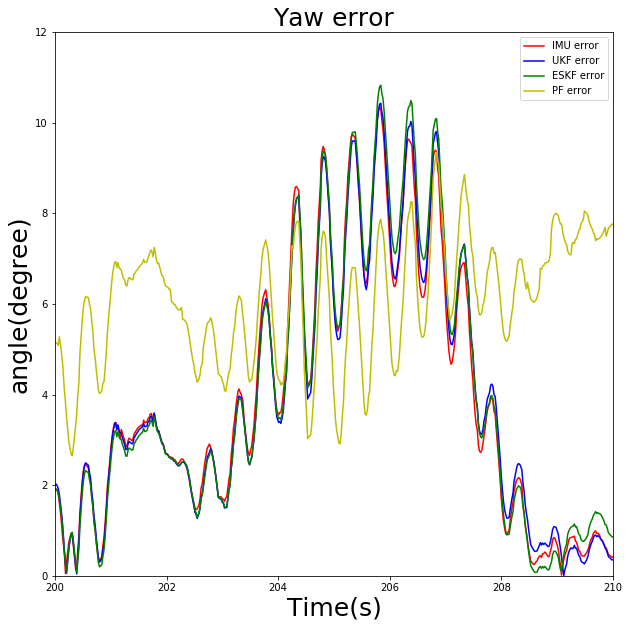
\includegraphics[width=0.7\textwidth]{figs/yaw.png}
	\caption{Filter comparison - error in yaw}
	\label{fig:ch:errorYaw}
\end{figure}


%%%%%%%% ch end %%%%%%%%%





%%%%%%%%%%%%%%%
\section{Sensor fusion mechanism}
The effect of fusing relative measurements through stochastic cloning was observed using the \gls{NCLT} dataset. \gls{GNSS} and Magnetometer data were used as absolute measurements and wheel odometry data were used as relative measurements. A 30 s \gls{GNSS} outage was simulated, and the error in the estimate was observed for the two instances; with and without fusing relative measurements. It was observed that with the integration of relative measurement data, the error remained bounded (see figure \ref{fig:pa:relativeMeasurements}).
\begin{figure}[h]
	\centering
    \begin{subfigure}{\textwidth}
        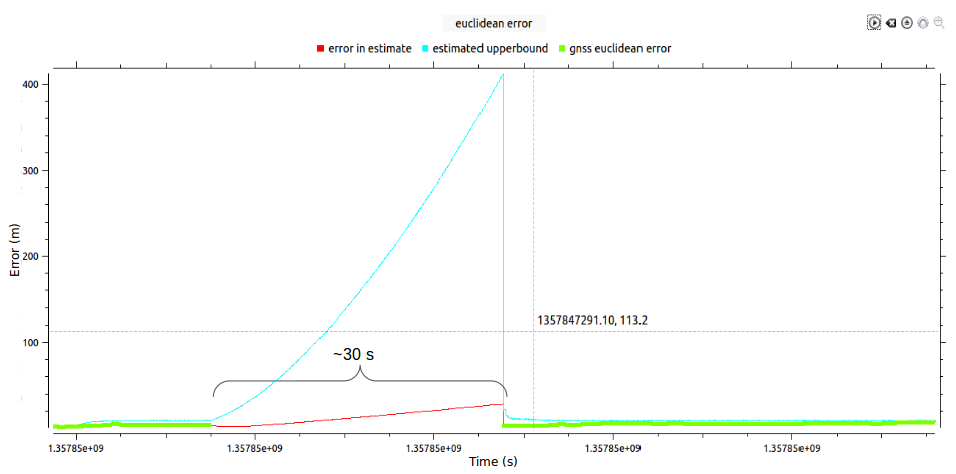
\includegraphics[width=\textwidth]{figs/euclidean-error-wo-rm.png}
        \caption{Euclidean error without relative measurements}
    \end{subfigure}
    \begin{subfigure}{\textwidth}
        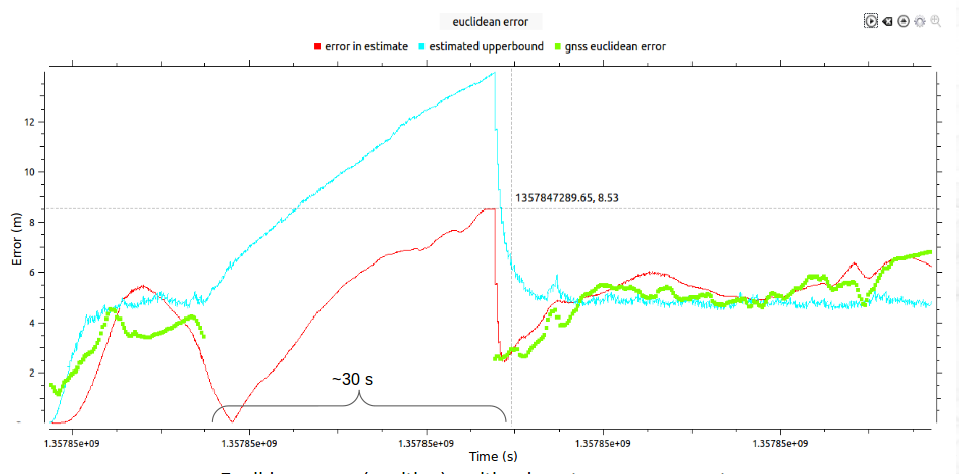
\includegraphics[width=\textwidth]{figs/euclidean-error-with-rm.png}
        \caption{Euclidean error with relative measurements}
    \end{subfigure}
    \caption[Effect of relative measurements]{Effect of relative measurements during a \gls{GNSS} interruption. Green: error in \gls{GNSS} measurements, Red: error in estimate, Cyan: estimated upper bound for the error.}
    \label{fig:pa:relativeMeasurements}
\end{figure}

Adding \gls{ZUPT} measurements has a significant effect on the accuracy of the yaw estimate, as seen from figure \ref{fig:pa:zuptYaw}. When \gls{ZUPT} measurements are applied, the yaw estimate error remains within the estimated error bounds (3$\sigma$ bounds), despite the fact that the magnetometer-estimated yaw is biased.
\begin{figure}[h]
	\centering
    \begin{subfigure}{\textwidth}
        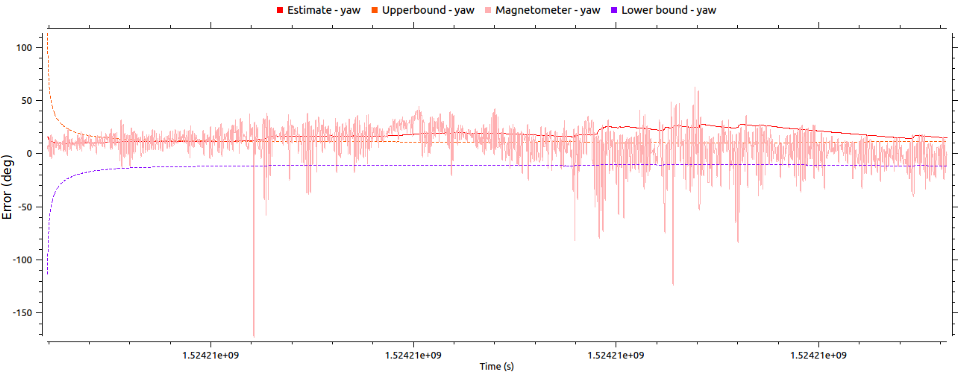
\includegraphics[width=\textwidth]{figs/yaw-without-zupt.png}
        \caption{Yaw estimate without \gls{ZUPT} measurements}
    \end{subfigure}
    \begin{subfigure}{\textwidth}
        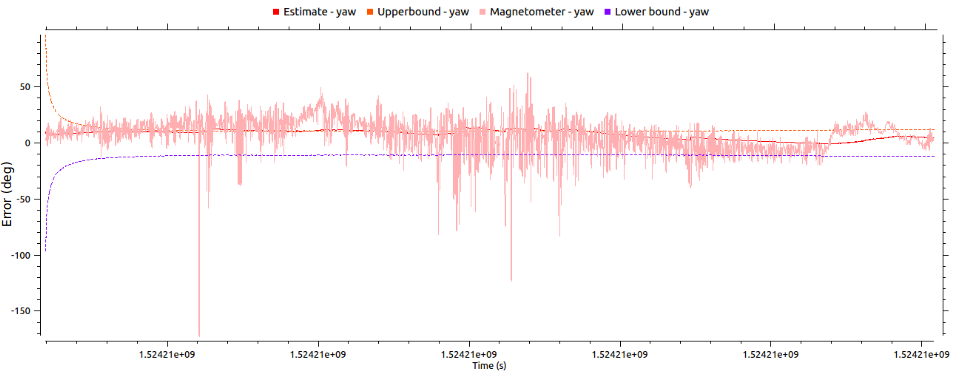
\includegraphics[width=\textwidth]{figs/yaw-with-zupt.png}
        \caption{Yaw estimate with \gls{ZUPT} measurements}
    \end{subfigure}
    \caption[Effect of \gls{ZUPT} measurements on the yaw estimate]{Effect of \gls{ZUPT} measurements on the yaw estimate. Pink: Magnetometer estimated yaw, Red: Filter output, Orange (dashed): Estimated upper bound of the error, Violet (dashed): Estimated lower bound of the error.}
    \label{fig:pa:zuptYaw}
\end{figure}







%%%%%%%%%%%% ra start %%%%%%%%%%%%%%%%%%%%

\section{Visual Odometry}
\label{sec:VisualOdometry}

Experiments were conducted using the \gls{KITTI} and \gls{KAIST} datasets on the \gls{ORBSLAM}. Images in the \gls{KITTI} odometry dataset are rectified images and the ones in the \gls{KAIST} dataset are non-rectified. Therefore, images should be rectified in system for the \gls{KAIST} dataset. Results in the subsequent discussion have been obtained using the \gls{KITTI} dataset. Coordinate axes, x, y and z refer to the coordinate axes of the initial camera frame (Coordinate frame of the camera, when the vehicle started moving).

When running \gls{ORBSLAM} algorithm, it creates a feature points map using the detected feature points (see figure \ref{fig:ra:detected_features}) and localize the vehicle in the feature map. Figure \ref{fig:ra:point_map} shows the estimated path of the vehicle in the map.
\begin{figure}[h]
	\centering
	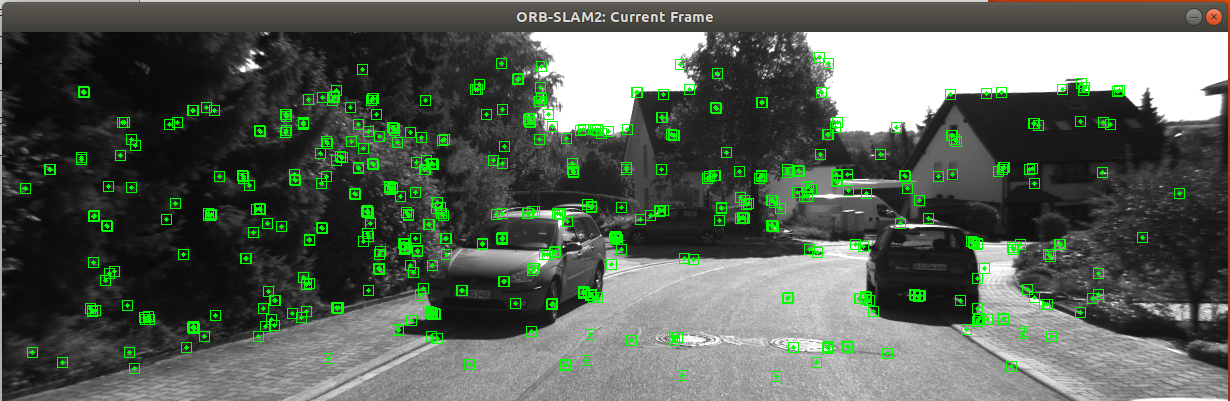
\includegraphics[width=\textwidth]{figs/detected_features.png}
	\vspace{-0.5cm}
	\caption[Detected feature points]{Feature points detected in a frame of \gls{KITTI} sequence 09 when running \gls{ORBSLAM}. Green colour squares indicate the feature points.}
	\label{fig:ra:detected_features}
	\vspace{0.5cm}
\end{figure}
\begin{figure}[h]
	\centering
	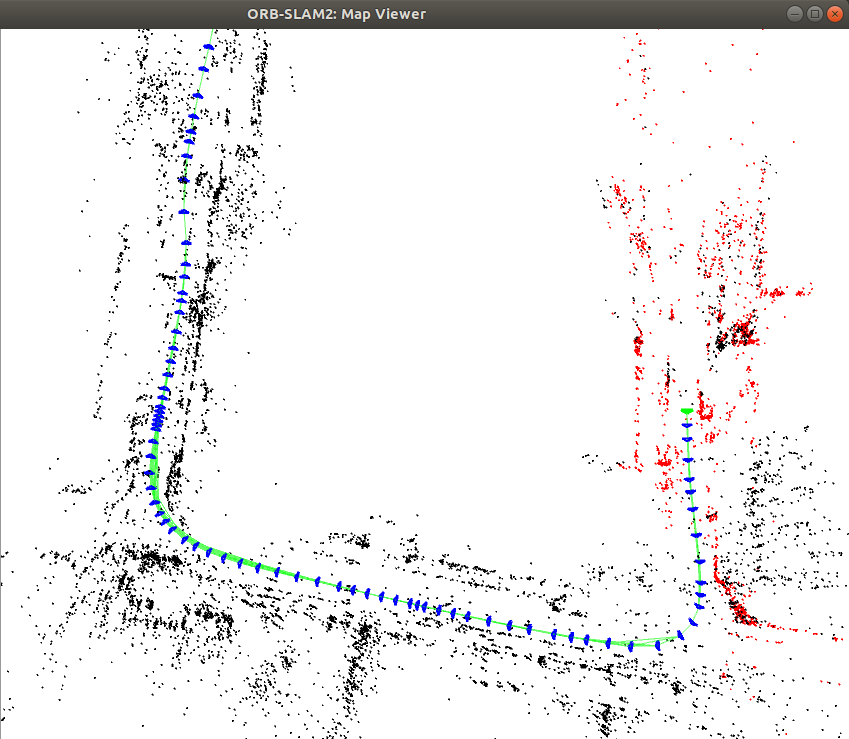
\includegraphics[width=\textwidth]{figs/path_pred.png}
	\vspace{-0.5cm}
	\caption[Map of feature points]{Part of the feature point map generated from \gls{ORBSLAM}, using \gls{KITTI} sequence 00. Estimated path of the vehicle is shown in green colour. Blue triangles show the pose of the camera, in the respective frames.}
	\label{fig:ra:point_map}
	\vspace{0.5cm}
\end{figure}

Figure \ref{fig:ra:xyz_error} shows the position error in the directions of x, y and z with the frame index, and figure \ref{fig:ra:rpy_error} shows the error in the orientation (roll, pitch and yaw) with the frame index. It can be observed that the total position error in a given direction increase with time due to the accumulation of the relative position errors in the estimate.
\begin{figure}[h]
	\centering
	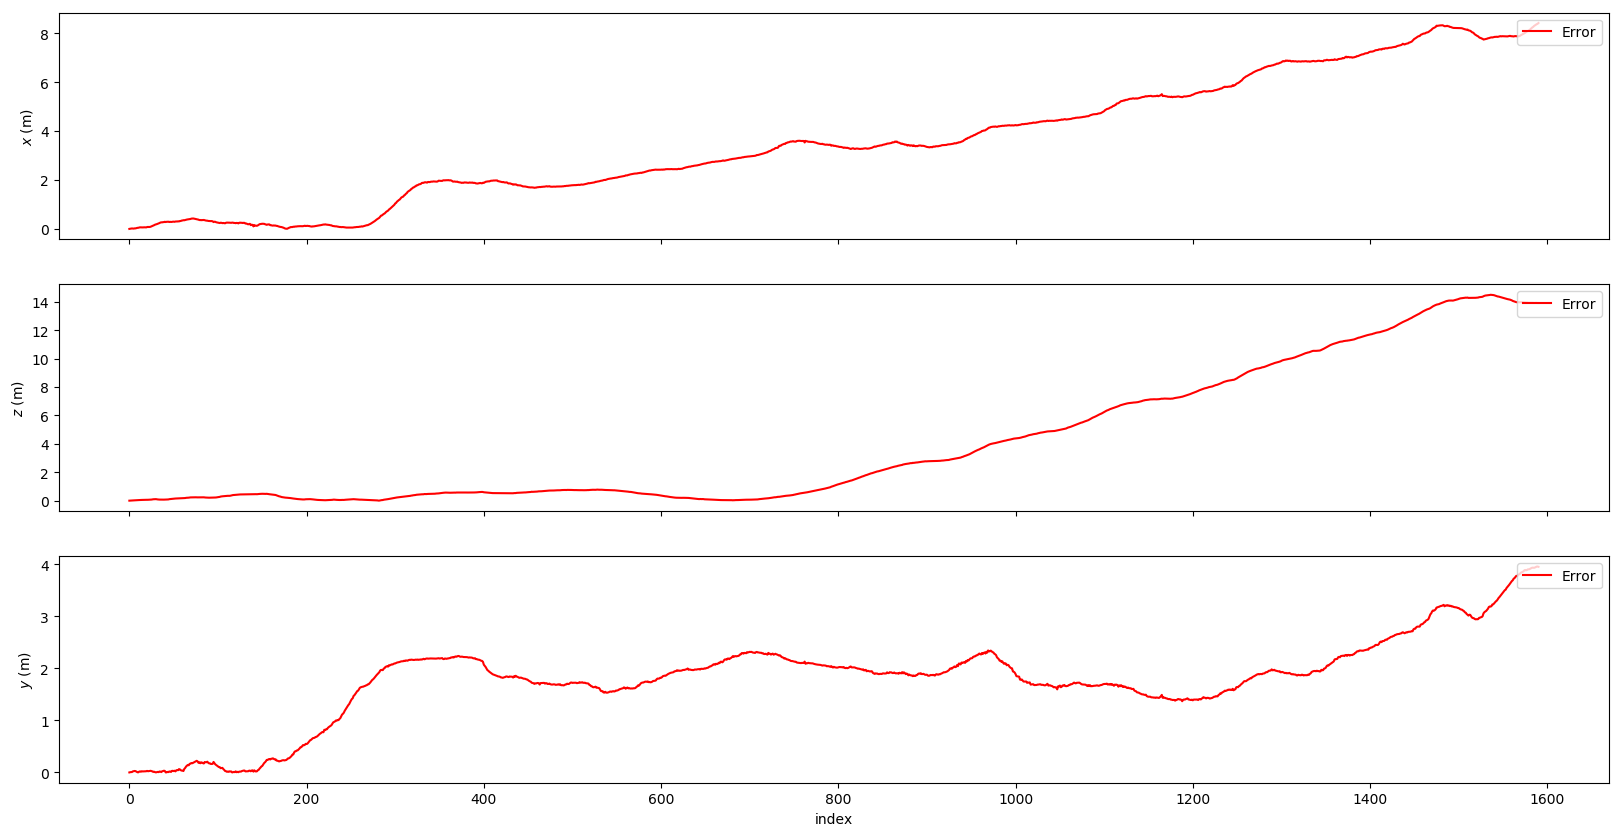
\includegraphics[ width=\textwidth]{figs/xyz_error.png}
	\vspace{-0.5cm}
	\caption[Positional error of \gls{ORBSLAM}]{Positional error of \gls{ORBSLAM} (\gls{KITTI} sequence 09)}
	\label{fig:ra:xyz_error}
	\vspace{0.5cm}
\end{figure}
\begin{figure}[h]
	\centering
	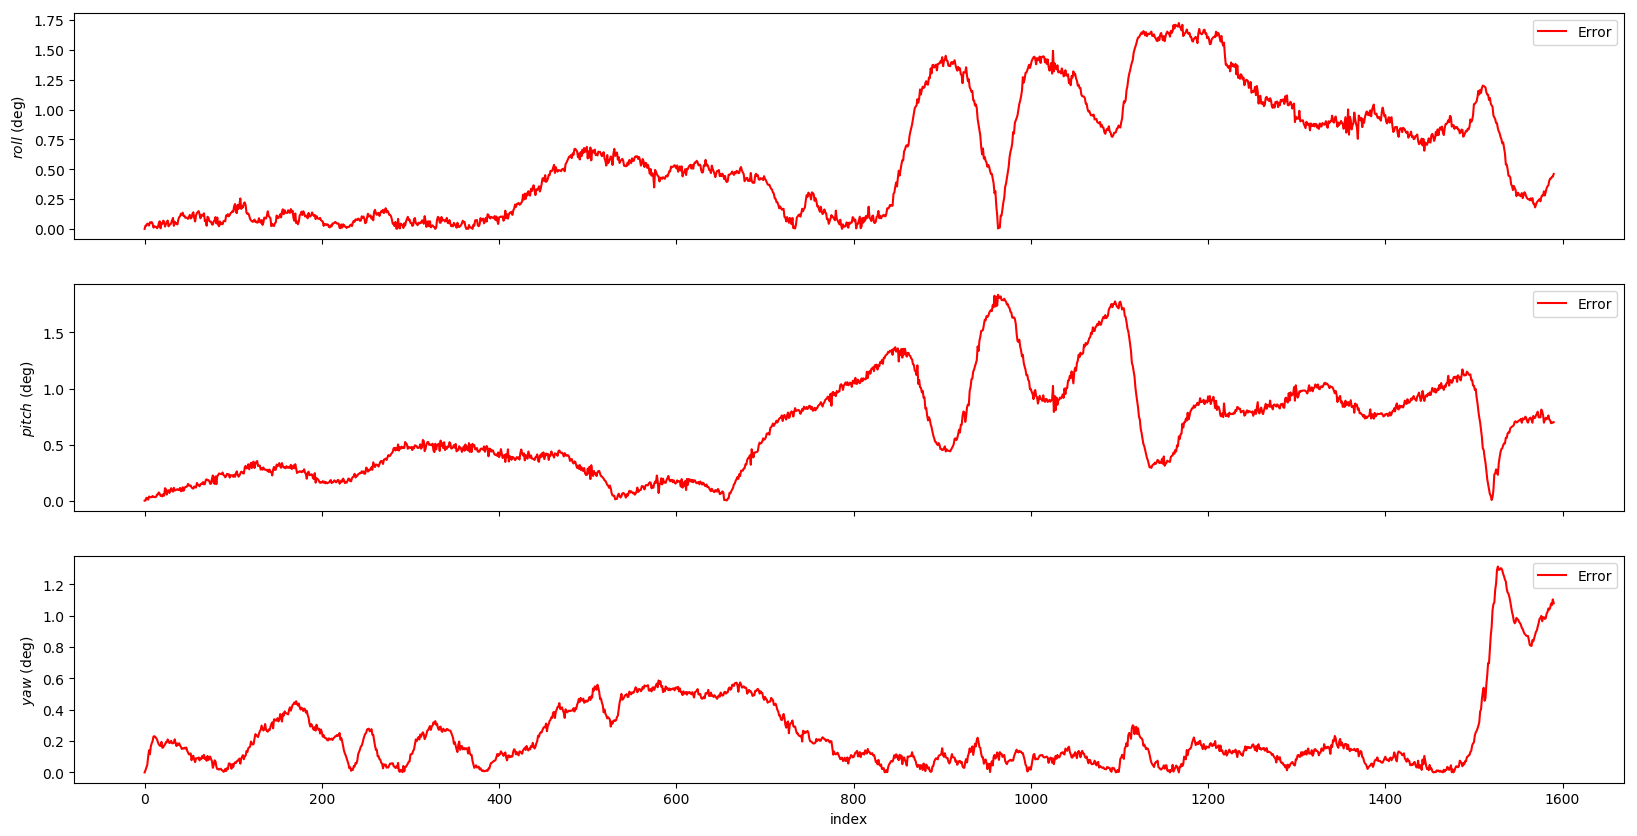
\includegraphics[ width=\textwidth]{figs/rpy_error.png}
	\vspace{-0.5cm}
	\caption[Rotational error of \gls{ORBSLAM}]{Rotational error of \gls{ORBSLAM} (\gls{KITTI} sequence 09)}
	\label{fig:ra:rpy_error}
	\vspace{0.5cm}
\end{figure}

In-order to test the effect of error accumulation, we subtracted the error of the previous frame, from the total error of the current frame, thereby removing the effect of accumulated error, for each frame. This revealed that the error in the relative position/orientation estimate of the algorithm is extremely low (within $\pm$0.1 m for position and $\pm0.2^o$ for orientation, for \gls{KITTI} dataset), which is desirable when using the output as a relative measurement in the fusion mechanism (see figures \ref{fig:ra:xyz_error_allred} and \ref{fig:ra:rpy_error_allred}).
\begin{figure}[h]
	\centering
	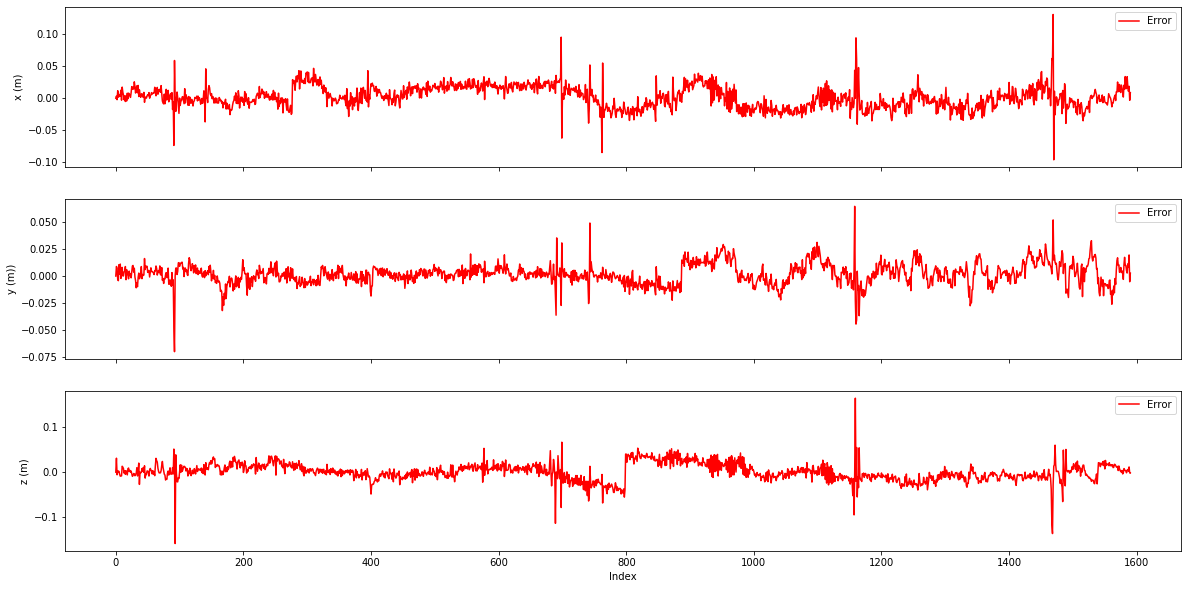
\includegraphics[width=\textwidth]{figs/xyz_error_allred.png}
	\vspace{-0.5cm}
	\caption{Positional error of \gls{ORBSLAM}, after removing the effect of error accumulation}
	\label{fig:ra:xyz_error_allred}
	\vspace{0.5cm}
\end{figure}
\begin{figure}[h]
	\centering
	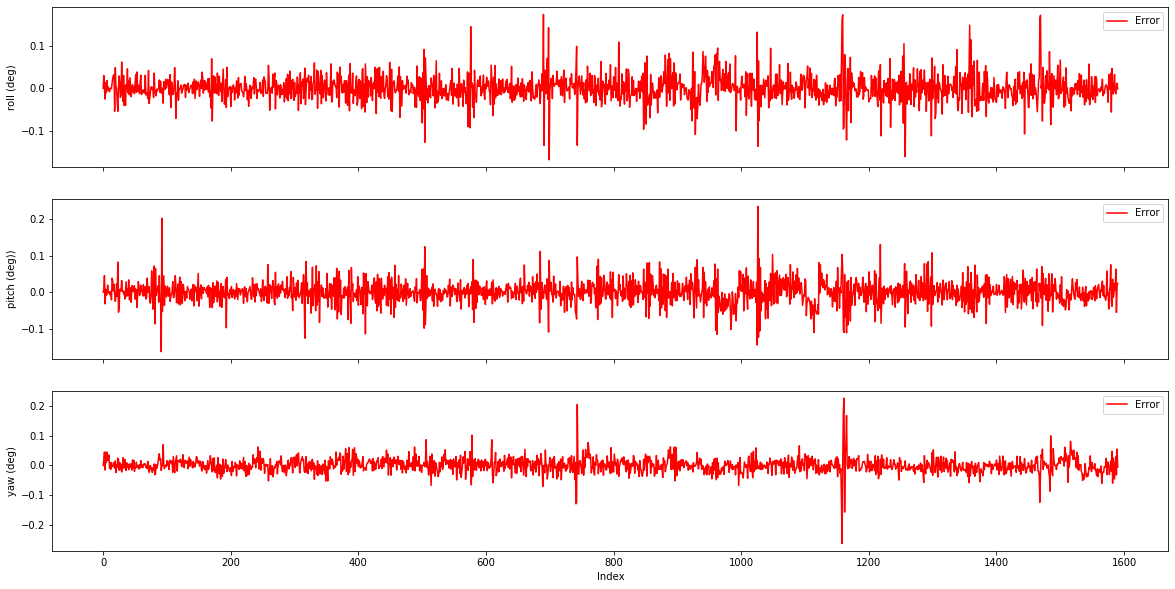
\includegraphics[ width=\textwidth]{figs/rpy_error_allred.png}
	\vspace{-0.5cm}
	\caption{Rotational error of \gls{ORBSLAM}, after removing the effect of error accumulation}
	\label{fig:ra:rpy_error_allred}
	\vspace{0.5cm}
\end{figure}

With the intention of obtaining insights for implementing an error covariance estimation mechanism for \gls{ORBSLAM}, a histogram was obtained by counting the number of feature points detected in a given frame. It appeared to be concentrated around 300 for the \gls{KITTI} dataset (figure \ref{fig:ra:matched_points}).
\begin{figure}[h]
	\centering
	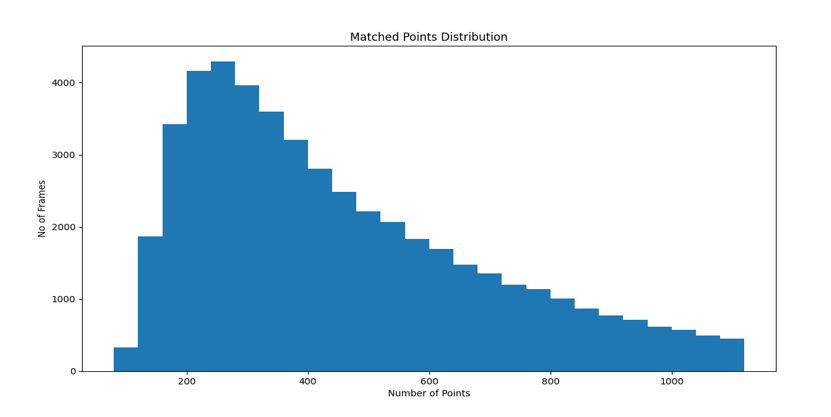
\includegraphics[ width=\textwidth]{figs/matched_points.png}
	\vspace{-0.5cm}
	\caption[Histogram of the number of matched points]{Histogram of the number of matched points. Vertical axis denotes the number of frames, with a given number of feature points detected.}
	\label{fig:ra:matched_points}
	\vspace{0.5cm}
\end{figure}

Furthermore, we calculated the average \gls{RMS} error obtained for a given number of matched points in a frame (see figure \ref{fig:ra:rms_error}), which showed that up to some optimal number, the \gls{RMS} error decreases with the number of matched points. However, beyond this point, it was observed that the \gls{RMS} error increases. A possible reason for this is the confusion caused by the large number of feature points (with similar features) detected very close to each other. When the number of detected features exceeds 1500, only the best 1500 features will be selected for the pose estimation mechanism, leaving the excess features unused. The saturation behaviour observed in the plot is a consequence of this.
\begin{figure}[h]
	\centering
	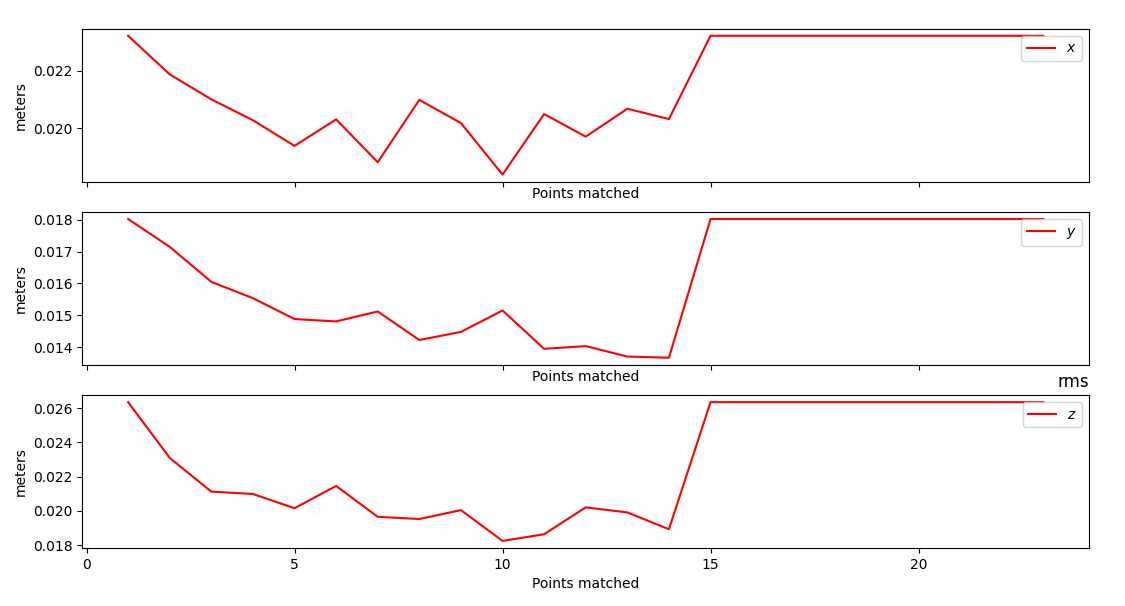
\includegraphics[ width=\textwidth]{figs/rms_error.png}
	\vspace{-0.5cm}
	\caption[Average \gls{RMS} error vs. the number of matched points]{Variation of average \gls{RMS} error, with the number of matched points (in hundreds)}
	\label{fig:ra:rms_error}
	\vspace{0.5cm}
\end{figure}


%%%%%%%%%%% ra end %%%%%%%%%%%%%%%%%%%%%%%








%%%%%%%%%%%%%%%% hi start %%%%%%%%%%%%%%%%%


\section{Lidar Odometry}
Following results were obtained using the \gls{KITTI} and \gls{KAIST} datasets. The frame of reference for the plots shown in the following discussion is the initial coordinate frame of the \gls{LiDAR} sensor, at the moment the vehicle started moving.

The \gls{LeGO-LOAM} algorithm creates a map of points through the map construction module and localize the vehicle within the map. Figure \ref{fig:ha:lidar_map} shows such a map and the predicted path of the vehicle in the map.
\begin{figure}[h]
	\centering
	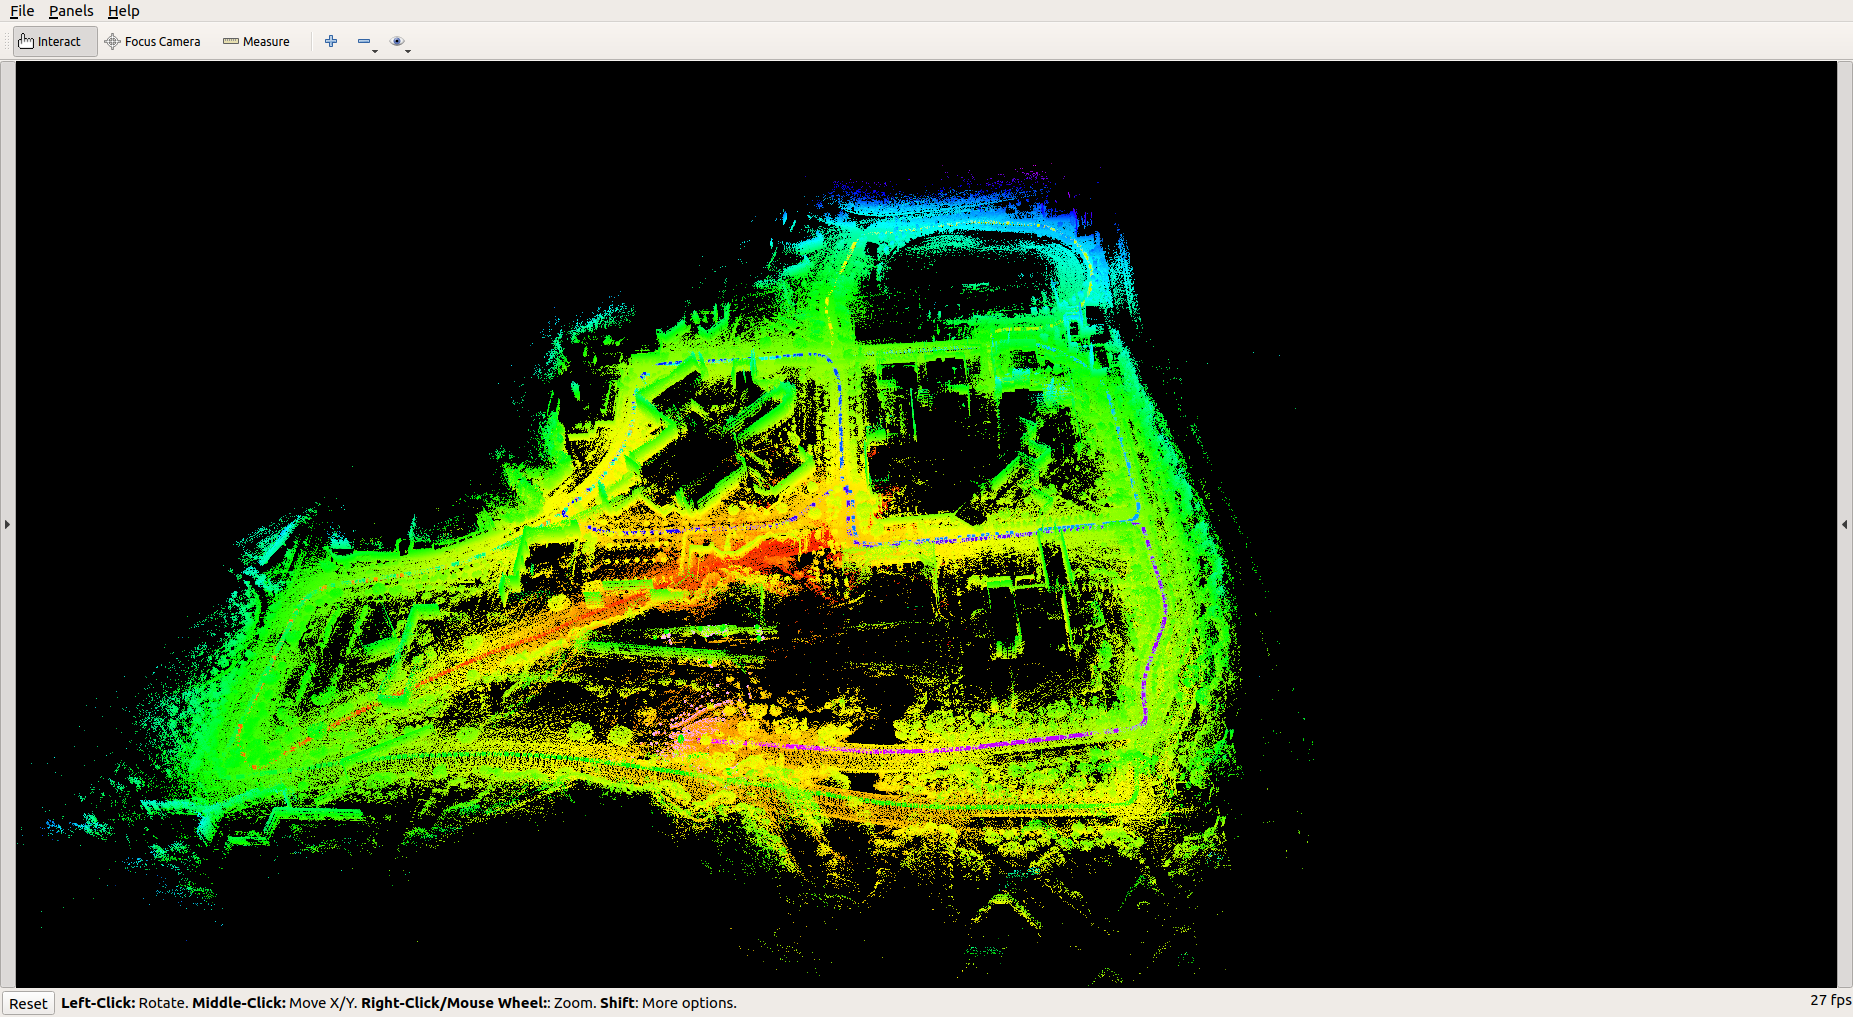
\includegraphics[width=\textwidth]{figs/rviz_lidar.png}
	\vspace{-0.2cm}
	\caption[\gls{LeGO-LOAM} generated \gls{SLAM} map using \gls{KAIST}dataset]{\gls{LeGO-LOAM} generated \gls{SLAM} map using \gls{KAIST}dataset. Coloured points are the \gls{LiDAR} point cloud points, based on their intensity level.}
	\label{fig:ha:lidar_map}
	\vspace{0.2cm}
\end{figure}

Figure \ref{fig:hi:xyz_error} shows the \gls{LeGO-LOAM} estimated position error in the directions of x, y and z, with the frame index and figure \ref{fig:hi:rpy_error} shows the error in roll, pitch and yaw with the frame index. It can be seen that, position error increase with time and reduces back to a lower value. The increase is caused by the error accumulation, while adding up the relative translations of the vehicle to obtain the overall position. The reduction in the error is a result of the system using loop closure global optimization method to optimize the path while building the map.

\begin{figure}[h]
	\centering
	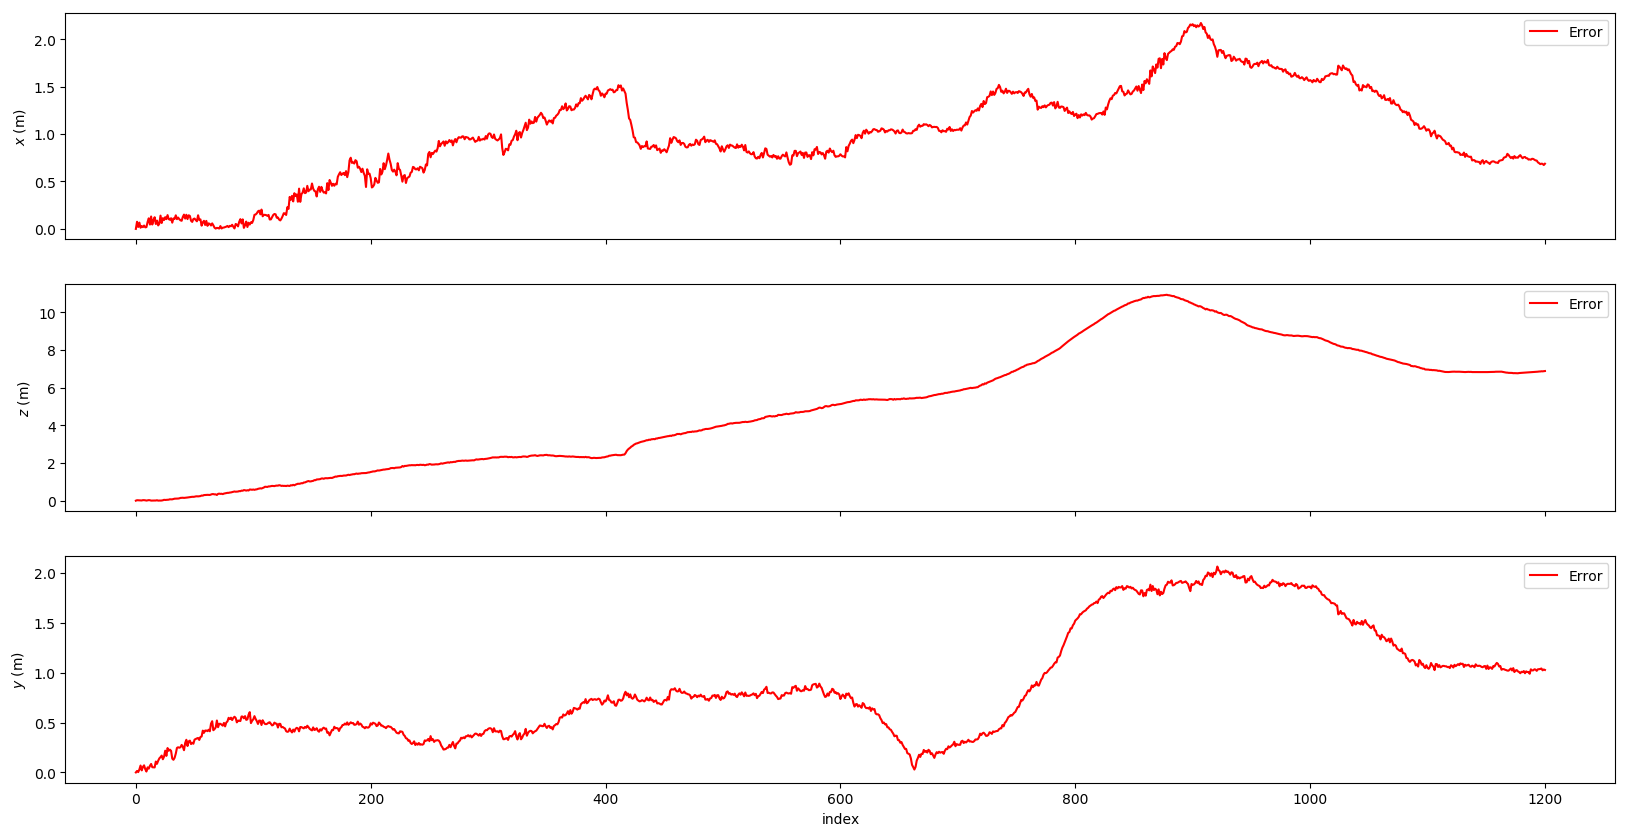
\includegraphics[ width=\textwidth]{figs/lidar_xyz_error.png}
	\vspace{-0.5cm}
	\caption{Error in x, y and z direction for \gls{KITTI} sequence 05}
	\label{fig:hi:xyz_error}
	\vspace{0.5cm}
\end{figure}

\begin{figure}[h]
	\centering
	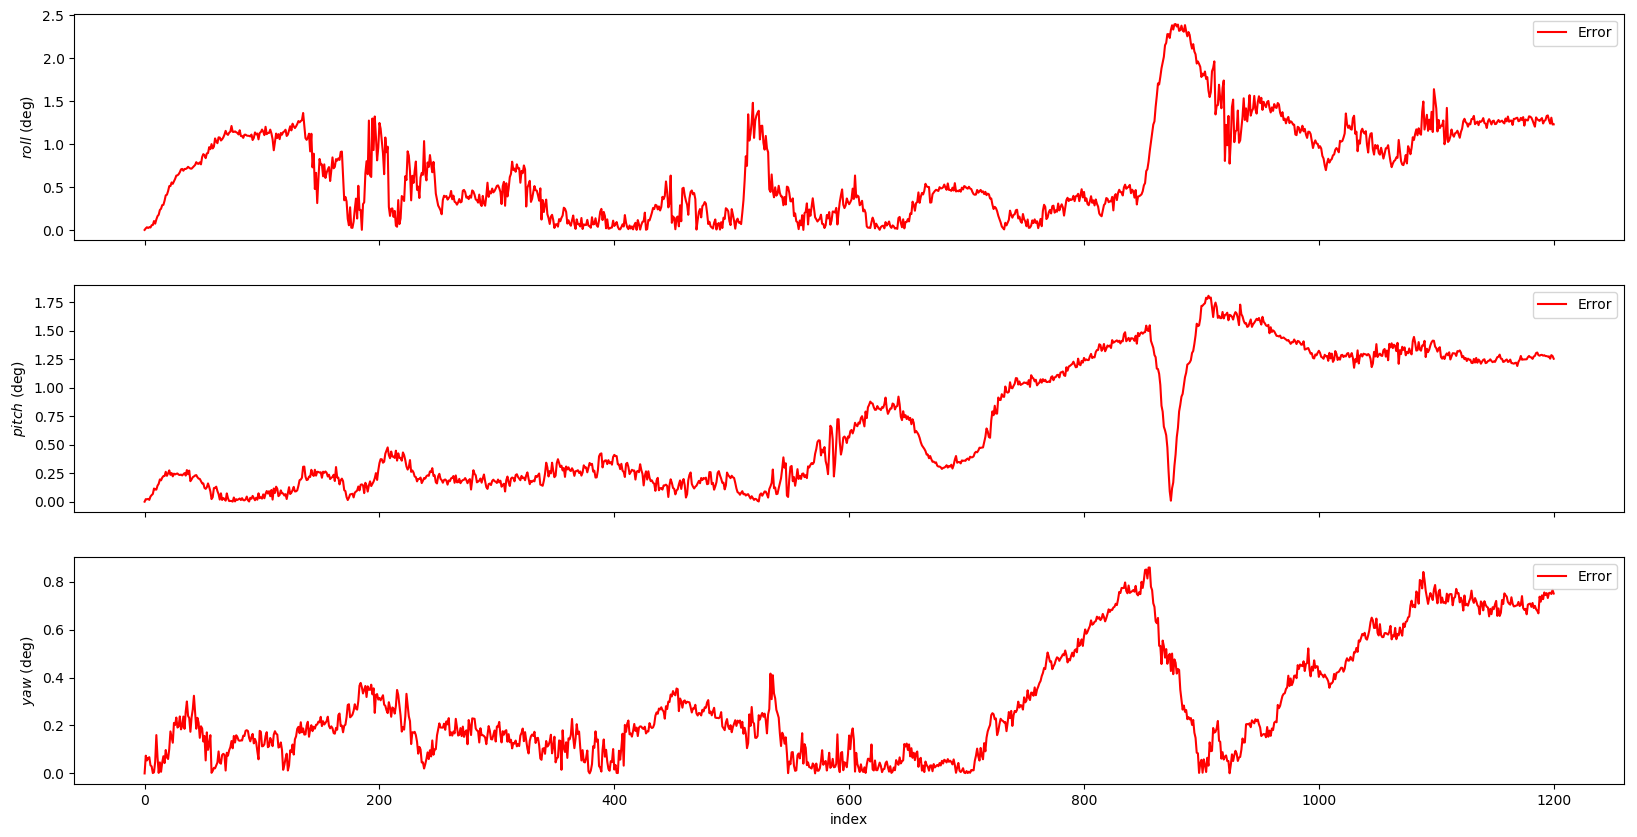
\includegraphics[ width=\textwidth]{figs/lidar_rpy_error.png}
	\vspace{-0.5cm}
	\caption{Error in roll, pitch and yaw for \gls{KITTI} sequence 05}
	\label{fig:hi:rpy_error}
	\vspace{0.5cm}
\end{figure}


%%%%%%%%%%%%%%%% hi end %%%%%%%%%%%%%%%%%%%%